\documentclass[10pt, conference, a4paper, compsocconf]{IEEEtran}
\usepackage{amsmath,amsxtra,amssymb,amsthm,latexsym,amscd,amsfonts}
\usepackage[utf8]{vietnam}
\usepackage[top=2.7cm, bottom=5.4cm, left=2.72cm, right=3.0cm]{geometry}
\headsep=0.7cm
\headheight=1.0cm
\footskip=1.0cm
\voffset=-0.74cm

\usepackage{fancyhdr}
\pagestyle{fancy}
\renewcommand{\sectionmark}[1]{\markright{\MakeUppercase{#1}}{}}
\renewcommand{\headrulewidth}{0pt}

\ifCLASSINFOpdf
\usepackage[pdftex]{graphicx}
\usepackage{pgfplots}
\pgfplotsset{compat=1.17}
\DeclareGraphicsExtensions{.pdf,.jpeg,.png,.jpg}
\else
\usepackage[dvips]{graphicx}
\DeclareGraphicsExtensions{.eps}
\fi

\usepackage{array}
\usepackage{url}
\usepackage{float}
\usepackage[caption=false,font=footnotesize]{subfig}
\usepackage{tikz}
\usetikzlibrary{arrows.meta,positioning,shapes.geometric}

\makeatletter
\def\ps@IEEEtitlepagestyle{%
\def\@oddhead{\centering{\mbox{\footnotesize{\textit{\;\;\;\; Bài tập lớn: Môn Phát triển phần mềm mã nguồn mở -- Đại học Sài Gòn, 5-6/04/2026}}}}%
\def\@evenhead{\centering{\mbox{\footnotesize{\textit{\;\;\;\; Bài tập lớn: Môn Phát triển phần mềm mã nguồn mở -- Đại học Sài Gòn, 5-6/04/2026}}}}}%
\def\@oddfoot{\scriptsize \thepage \hfil }%
\def\@evenfoot{\scriptsize \hfil \thepage}
}
}
\makeatother

\begin{document}
\pagenumbering{arabic}
\fontsize{10}{12}
\selectfont

\fancyhead[RE,LO]{\centering{\footnotesize{\textit{Bài tập lớn: Môn Phát triển phần mềm mã nguồn mở -- Đại học Sài Gòn, 5-6/04/2026}}}}

\title{SmartDoc AI: Hệ thống hỏi đáp tài liệu thông minh\\với RAG và Chain-of-RAG}

\author{
    \IEEEauthorblockN{Nhóm 17\IEEEauthorrefmark{1}}
    \IEEEauthorblockA{\IEEEauthorrefmark{1}Khoa Công nghệ Thông tin, Trường Đại học Sài Gòn}
    \IEEEauthorblockA{Các thành viên trong nhóm: }
    
    \IEEEauthorblockA{Nguyễn Thanh Thịnh, Huỳnh Đức Huy, Nguyễn Hùng}
    \IEEEauthorblockA{Cao Minh Thuận, Hoàng Luân, Nguyễn Thành Nam}
}
\maketitle

\begin{abstract}
Báo cáo trình bày quá trình thiết kế, hiện thực và đánh giá hệ thống SmartDoc AI --- trợ lý hỏi đáp tài liệu chạy cục bộ, phục vụ môi trường giáo dục. Hệ thống vận hành theo hướng \textit{local-first} với Ollama (\texttt{qwen2.5:7b}), FAISS, BM25 và cross-encoder reranking. Nhóm hiện thực 10 yêu cầu phát triển arranged theo 4 nhóm: (i) \textbf{Core Features} --- hỗ trợ DOCX, OCR, lịch sử hội thoại, xóa dữ liệu; (ii) \textbf{Retrieval Optimization} --- chunking linh hoạt, hybrid search (Vector + BM25), cross-encoder reranking; (iii) \textbf{User Experience} --- citation/source tracking, multi-document với metadata filtering; (iv) \textbf{Advanced Intelligence} --- conversational RAG với follow-up rewriting, Self-RAG với self-evaluation và confidence scoring, cùng Chain-of-RAG (CoRAG) bổ sung. Kiến trúc phân lớp Views--Controllers--Services--Models kết hợp Strategy Pattern cho phép chuyển đổi linh hoạt giữa các chiến lược. Kết quả thực nghiệm cho thấy hybrid retrieval tăng độ đầy đủ 10\% so với vector-only, trong khi Self-RAG và CoRAG cải thiện rõ rệt chất lượng trả lời cho truy vấn phức tạp đa bước.
\end{abstract}

\begin{IEEEkeywords}
RAG; Self-RAG; Chain-of-RAG; Ollama; FAISS; BM25; Cross-Encoder; Streamlit
\end{IEEEkeywords}

\IEEEpeerreviewmaketitle

\section{Giới thiệu và công trình liên quan}

Trong bối cảnh học tập và nghiên cứu, sinh viên thường làm việc với nhiều tài liệu rời rạc (PDF, DOCX, TXT) và cần truy xuất thông tin theo ngữ cảnh cụ thể. Các chatbot tổng quát thường trả lời ``đúng ngữ pháp nhưng sai nguồn'', trong khi tra cứu thủ công tốn thời gian. Từ nhu cầu đó, SmartDoc AI được xây dựng như một trợ lý hỏi đáp tài liệu chạy hoàn toàn cục bộ, tập trung vào tính riêng tư dữ liệu, chi phí vận hành thấp và khả năng mở rộng theo module.

Hệ thống cung cấp giao diện Streamlit cho người dùng cuối, tối ưu hóa cho môi trường local/edge: không yêu cầu GPU, chạy trên CPU phổ thông với RAM trung bình, có cơ chế fallback khi tài nguyên hạn chế.

Nhóm tham khảo các công trình nền tảng: LangChain~\cite{langchain} cho orchestration, FAISS~\cite{faiss} cho ANN retrieval, BM25~\cite{bm25} cho keyword retrieval, Cross-Encoder reranking~\cite{crossencoder}, Ollama~\cite{ollama} cho local LLM serving. Thiết kế Strategy Pattern cho phép so sánh trực tiếp Standard RAG và Chain-of-RAG trong cùng một hệ thống.

\section{Thiết kế hệ thống}

\subsection{Kiến trúc tổng thể}

SmartDoc AI tổ chức theo phân lớp: \textit{Views} (Streamlit screens), \textit{Controllers} (điều phối, validate), \textit{Services} (RAG pipeline, retrieval, LLM), và \textit{Models/Utils} (thực thể dữ liệu, exceptions, logger). Giao diện Streamlit là kênh truy cập chính, đảm bảo logic nghiệp vụ nhất quán.

\begin{figure}[t]
\centering
\resizebox{0.95\columnwidth}{!}{%
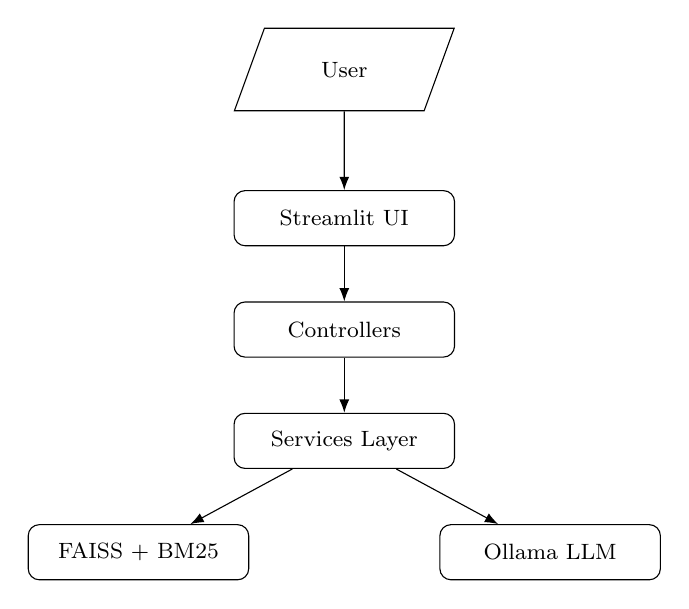
\begin{tikzpicture}[
  node distance=5mm,
  >=Latex,
  box/.style={rectangle, rounded corners, draw=black, align=center, minimum width=2.8cm, minimum height=0.7cm, font=\footnotesize},
  io/.style={trapezium, trapezium left angle=70, trapezium right angle=110, draw=black, align=center, minimum width=2.8cm, minimum height=0.7cm, font=\footnotesize}
]
\node[io] (user) {User};
\node[box, below=10mm of user] (streamlit) {Streamlit UI};
\node[box, below=7mm of streamlit] (ctrl) {Controllers};
\node[box, below=7mm of ctrl] (services) {Services Layer};
\node[box, below left=7mm and -2mm of services] (stores) {FAISS + BM25};
\node[box, below right=7mm and -2mm of services] (ollama) {Ollama LLM};

\draw[->] (user) -- (streamlit);
\draw[->] (streamlit) -- (ctrl);
\draw[->] (ctrl) -- (services);
\draw[->] (services) -- (stores);
\draw[->] (services) -- (ollama);
\end{tikzpicture}
}
\caption{Kiến trúc phân lớp của hệ thống}
\label{fig:architecture}
\end{figure}

Điểm nổi bật là áp dụng \textbf{Strategy Pattern} cho RAG pipeline: interface \texttt{AbstractRAGStrategy} định nghĩa \texttt{process\_query\_stream()}, với hai cài đặt cụ thể là \texttt{StandardRAGStrategy} và \texttt{ChainOfRAGStrategy}. Người dùng chuyển đổi chiến lược qua giao diện mà không ảnh hưởng các thành phần khác.

\subsection{Pipeline tổng quan}

Luồng xử lý chính gồm: (1) nạp tài liệu bằng loader phù hợp định dạng; (2) chia văn bản thành chunk có chồng lấn; (3) sinh embedding và lập chỉ mục FAISS, đồng thời dựng BM25 retriever; (4) truy hồi top-$k$ theo chiến lược đã chọn; (5) dựng prompt có ngữ cảnh và gọi Ollama; (6) trả kết quả kèm trích dẫn nguồn. Các tham số mặc định: \texttt{chunk\_size=1000}, \texttt{chunk\_overlap=100}, \texttt{retrieval\_k=3}, model \texttt{qwen2.5:7b}.

\section{Triển khai các yêu cầu phát triển}

Nhóm hiện thực 10 yêu cầu + OCR, được gộp theo 4 nhóm logic. Bảng~\ref{tab:feature-summary} tổng hợp toàn bộ tính năng đã triển khai.

\begin{table}[t]
\renewcommand{\arraystretch}{1.1}
\caption{Tổng hợp tính năng đã triển khai}
\label{tab:feature-summary}
\centering
\resizebox{\columnwidth}{!}{%
\begin{tabular}{|l|l|c|}
\hline
\textbf{Nhóm / Tính năng} & \textbf{Công nghệ chính} & \textbf{Yêu cầu} \\
\hline
\multicolumn{3}{|l|}{\textit{Core Features}} \\
\hline
DOCX support & DocxLoader, Factory Pattern & 8.2.1 \\
\hline
OCR tài liệu scan & Tesseract, pdf2image & Bổ sung \\
\hline
Lịch sử hội thoại & ChatHistory model, persistence & 8.2.2 \\
\hline
Xóa history + vector store & Confirmation dialog, clear APIs & 8.2.3 \\
\hline
\multicolumn{3}{|l|}{\textit{Retrieval Optimization}} \\
\hline
Chunk strategy tuning & Benchmark 4 configs, UI slider & 8.2.4 \\
\hline
Hybrid search (Vector + BM25) & Ensemble retriever, dedup & 8.2.7 \\
\hline
Cross-encoder reranking & ms-marco-MiniLM-L-6-v2 & 8.2.9 \\
\hline
\multicolumn{3}{|l|}{\textit{User Experience}} \\
\hline
Citation / source tracking & get\_citation(), source renderer & 8.2.5 \\
\hline
Multi-doc + metadata filter & Upload nhiều file, filter UI & 8.2.8 \\
\hline
\multicolumn{3}{|l|}{\textit{Advanced Intelligence}} \\
\hline
Conversational RAG & Follow-up rewrite, context window & 8.2.6 \\
\hline
Advanced RAG (Self-RAG) & Self-eval, rewrite, multi-hop, confidence & 8.2.10 \\
\hline
Chain-of-RAG (CoRAG) & Query dispatch, entity, chain & Bổ sung \\
\hline
\end{tabular}
}
\end{table}

\subsection{Core Features: DOCX, OCR, History, Clear}

\textbf{DOCX support (8.2.1):} Áp dụng Factory Pattern qua \texttt{DocumentLoaderFactory} với map extension $\to$ loader class (\texttt{PDFPlumberLoader}, \texttt{DocxLoader}, \texttt{TextLoader}). Khi tải file, factory tự chọn loader phù hợp dựa trên extension, đảm bảo text extraction chính xác cho từng định dạng.

\textbf{OCR tài liệu scan:} Tích hợp \texttt{ocr\_util.py} sử dụng Tesseract và pdf2image để xử lý tài liệu scan chất lượng thấp. Người dùng bật/tắt OCR qua giao diện; khi bật, các định dạng ảnh (.png, .jpg) cũng được chấp nhận upload. Hệ thống chuyển trang PDF thành ảnh, nhận dạng OCR, rồi đưa qua chunking pipeline bình thường.

\textbf{Lịch sử hội thoại (8.2.2):} Model \texttt{ChatHistory} quản lý danh sách \texttt{ChatMessage} với ngưỡng \texttt{max\_history=50}. Lịch sử được persist ra đĩa qua \texttt{persistence\_service.py}, khôi phục tự động khi session Streamlit bị reset. Sidebar hiển thị đầy đủ câu hỏi và câu trả lời đã gửi.

\textbf{Xóa dữ liệu (8.2.3):} Hai nút ``Clear Chat History'' và ``Clear Vector Store'' trong sidebar, mỗi nút yêu cầu confirmation checkbox trước khi thực hiện. Clear vector store đồng thời xóa FAISS index, metadata và session state, đảm bảo hệ thống trở trạng thái sạch.

\subsection{Retrieval Optimization: Chunking, Hybrid, Reranking}

\textbf{Chunk strategy tuning (8.2.4):} Giao diện Settings cung cấp slider cho \texttt{chunk\_size} (500--2000) và \texttt{chunk\_overlap} (50--200). Hàm \texttt{benchmark\_chunk\_configs()} re-chunk toàn bộ tài liệu đã nạp với 4 cấu hình (500/50, 1000/100, 1500/100, 2000/200), đo proxy accuracy và thời gian xử lý. Kết quả cho thấy cấu hình 1000/100 đạt cân bằng tốt nhất (accuracy 0.79, latency 2.5s).

\textbf{Hybrid search (8.2.7):} Kết hợp vector retrieval (FAISS) và keyword retrieval (BM25) qua ensemble retriever. Vector search xếp hạng theo cosine similarity:
\begin{equation}
\mathrm{sim}(q, d) = \frac{\mathbf{q} \cdot \mathbf{d}}{\|\mathbf{q}\|\,\|\mathbf{d}\|}
\end{equation}
Hệ thống merge hai danh sách ứng viên, loại trùng theo hash nội dung, rồi cắt top-$k$. Cách làm này cân bằng giữa truy hồi ngữ nghĩa (cho câu hỏi diễn đạt lại) và truy hồi từ khóa (cho câu hỏi chứa tên riêng, mã số, thuật ngữ đặc thù).

\textbf{Cross-encoder reranking (8.2.9):} Lazy-load \texttt{cross-encoder/ms-marco-MiniLM-L-6-v2} đánh giá lại relevance của từng chunk đã truy hồi. Cross-encoder encode đồng thời query và document, cho phép modeling tương tác phức tạp hơn bi-encoder thuần. Đổi lại, độ trễ tăng từ 2.5s lên 3.0s do cần forward pass qua model cho mỗi cặp query-document.

\subsection{User Experience: Citation, Multi-document}

\textbf{Citation/source tracking (8.2.5):} Model \texttt{Document} cung cấp \texttt{get\_citation()} trả về chuỗi dạng ``[filename, page X]''. Giao diện hiển thị trích dẫn trong expander ``View Sources'', cho phép xem context gốc và highlight đoạn được sử dụng. Metadata gồm \texttt{source}, \texttt{source\_file}, \texttt{file\_type}, \texttt{chunk\_index}, \texttt{chunk\_start/end}.

\textbf{Multi-document + metadata filtering (8.2.8):} Hỗ trợ upload nhiều file PDF/DOCX/TXT cùng lúc. Mỗi file được gắn metadata riêng (tên file, ngày upload, loại, số chunk). Giao diện retrieval settings cho phép lọc theo nguồn file hoặc file type. Câu trả lời hiển thị rõ nguồn từ document nào.

\subsection{Advanced Intelligence: Conversational RAG, Self-RAG, CoRAG}

\textbf{Conversational RAG (8.2.6):} Hệ thống lưu lịch sử hội thoại và sử dụng cửa sổ ngữ cảnh gần nhất để xử lý follow-up questions. Khi phát hiện câu hỏi tiếp theo (ví dụ: ``Còn về phần đó thì sao?''), controller thực hiện rewrite truy vấn dựa trên ngữ cảnh hội thoại trước đó, kết hợp lịch sử vào prompt để LLM tham chiếu câu trả lời trước.

\subsubsection{Advanced RAG --- Self-RAG (8.2.10)}

Self-RAG là yêu cầu cốt lõi của Task 10, triển khai 4 tính năng: (1) \textit{Self-evaluation} --- LLM tự đánh giá câu trả lời theo relevance, completeness, accuracy; (2) \textit{Query rewriting} --- tự động cải thiện câu hỏi trước khi retrieval; (3) \textit{Multi-hop reasoning} --- truy vấn phức tạp được phân tách và truy hồi nhiều bước; (4) \textit{Confidence scoring} --- đánh giá mức tin cậy (HIGH/MEDIUM/LOW) kèm justification.

\begin{figure}[t]
\centering
\resizebox{0.95\columnwidth}{!}{%
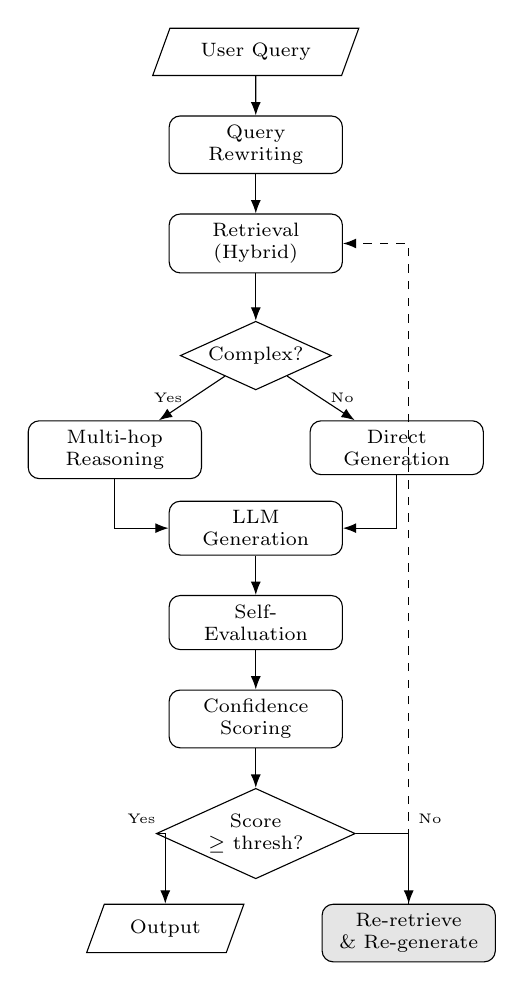
\begin{tikzpicture}[
  node distance=4mm and 3mm,
  >=Latex,
  box/.style={rectangle, rounded corners, draw=black, align=center, minimum width=2.2cm, minimum height=0.6cm, font=\scriptsize},
  decision/.style={diamond, draw=black, align=center, aspect=2.2, inner sep=1pt, font=\scriptsize},
  io/.style={trapezium, trapezium left angle=70, trapezium right angle=110, draw=black, align=center, minimum width=2cm, minimum height=0.6cm, font=\scriptsize}
]
\node[io] (query) {User Query};
\node[box, below=5mm of query] (rewrite) {Query\\Rewriting};
\node[box, below=5mm of rewrite] (retrieve) {Retrieval\\(Hybrid)};
\node[decision, below=6mm of retrieve] (complex) {Complex?};
\node[box, below left=6mm and 2mm of complex] (multihop) {Multi-hop\\Reasoning};
\node[box, below right=6mm and 2mm of complex] (direct) {Direct\\Generation};
\node[box, below=14mm of complex] (generate) {LLM\\Generation};
\node[box, below=5mm of generate] (selfeval) {Self-\\Evaluation};
\node[box, below=5mm of selfeval] (confidence) {Confidence\\Scoring};
\node[decision, below=5mm of confidence] (check) {Score\\$\geq$ thresh?};
\node[io, below left=6mm and 2mm of check] (output) {Output};
\node[box, fill=gray!20, below right=6mm and 2mm of check] (reregen) {Re-retrieve\\\& Re-generate};

\draw[->] (query) -- (rewrite);
\draw[->] (rewrite) -- (retrieve);
\draw[->] (retrieve) -- (complex);
\draw[->] (complex) -- node[left, font=\tiny]{Yes} (multihop);
\draw[->] (complex) -- node[right, font=\tiny]{No} (direct);
\draw[->] (multihop) |- (generate);
\draw[->] (direct) |- (generate);
\draw[->] (generate) -- (selfeval);
\draw[->] (selfeval) -- (confidence);
\draw[->] (confidence) -- (check);
\draw[->] (check) -| node[above left, font=\tiny]{Yes} (output);
\draw[->] (check) -| node[above right, font=\tiny]{No} (reregen);
\draw[->, dashed] (reregen) |- (retrieve);
\end{tikzpicture}
}
\caption{Flowchart Self-RAG pipeline}
\label{fig:selfrag-flow}
\end{figure}

Hình~\ref{fig:selfrag-flow} minh họa flow Self-RAG. Khi người dùng bật toggle \texttt{Self-RAG} trong Settings, controller gọi \texttt{process\_query\_with\_self\_rag()}: truy vấn đi qua rewriting, retrieval, multi-hop (nếu phức tạp), generation, rồi self-evaluation. Confidence score dưới ngưỡng sẽ kích hoạt re-retrieve và re-generate. UI hiển thị confidence (\%), level và self-evaluation justification.

\subsubsection{Chain-of-RAG --- CoRAG (Bổ sung)}

CoRAG là phần mở rộng bổ sung, triển khai pipeline nhiều bước với query dispatch và entity tracking:

\begin{figure}[t]
\centering
\resizebox{0.95\columnwidth}{!}{%
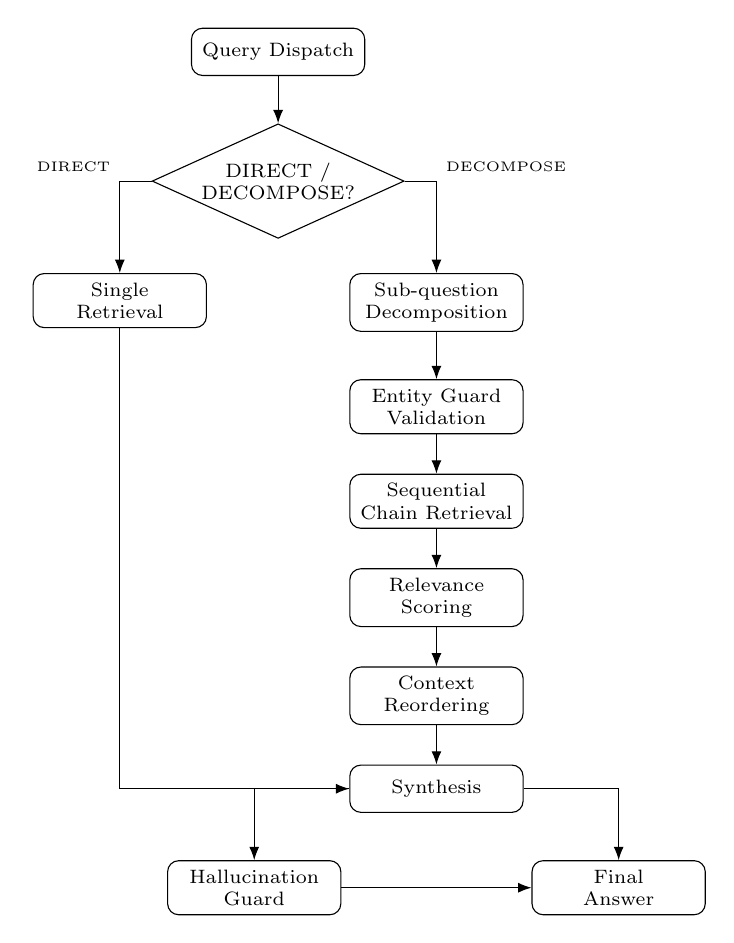
\begin{tikzpicture}[
  node distance=4mm,
  >=Latex,
  box/.style={rectangle, rounded corners, draw=black, align=center, minimum width=2.2cm, minimum height=0.6cm, font=\scriptsize},
  decision/.style={diamond, draw=black, align=center, aspect=2.2, inner sep=1pt, font=\scriptsize},
]
\node[box] (dispatch) {Query Dispatch};
\node[decision, below=6mm of dispatch] (type) {DIRECT /\\DECOMPOSE?};
\node[box, below left=8mm and 1mm of type] (direct) {Single\\Retrieval};
\node[box, below right=8mm and 1mm of type] (decomp) {Sub-question\\Decomposition};
\node[box, below=6mm of decomp] (entity) {Entity Guard\\Validation};
\node[box, below=5mm of entity] (chain) {Sequential\\Chain Retrieval};
\node[box, below=5mm of chain] (score) {Relevance\\Scoring};
\node[box, below=5mm of score] (reorder) {Context\\Reordering};
\node[box, below=5mm of reorder] (synth) {Synthesis};
\node[box, below left=6mm and 1mm of synth] (guard) {Hallucination\\Guard};
\node[box, below right=6mm and 1mm of synth] (output) {Final\\Answer};

\draw[->] (dispatch) -- (type);
\draw[->] (type) -| node[above left, font=\tiny]{DIRECT} (direct);
\draw[->] (type) -| node[above right, font=\tiny]{DECOMPOSE} (decomp);
\draw[->] (direct) |- (synth);
\draw[->] (decomp) -- (entity);
\draw[->] (entity) -- (chain);
\draw[->] (chain) -- (score);
\draw[->] (score) -- (reorder);
\draw[->] (reorder) -- (synth);
\draw[->] (synth) -| (guard);
\draw[->] (synth) -| (output);
\draw[->] (guard) -- (output);
\end{tikzpicture}
}
\caption{Flowchart CoRAG pipeline}
\label{fig:corag-flow}
\end{figure}

\begin{enumerate}
\item \textbf{Query Dispatch}: LLM phân tích cấu trúc câu hỏi, phân loại thành DIRECT (đơn giản) hoặc DECOMPOSE (phức tạp). Đồng thời trích xuất entities bằng regex kết hợp LLM.
\item \textbf{Sub-question decomposition}: Nếu DECOMPOSE, truy vấn được tách thành 2--4 câu hỏi con, mỗi câu hỏi được validate (Entity Guard).
\item \textbf{Sequential chain}: Mỗi câu hỏi con được truy hồi riêng, kết quả tích lũy dần. Cơ chế \textbf{early exit} khi entity coverage đạt 70\%.
\item \textbf{Semantic relevance}: Đánh giá bằng cosine similarity kết hợp word overlap:
\begin{equation}
R_{\mathrm{blend}} = \alpha \cdot \max_{s \in S}\cos(\mathbf{q}, \mathbf{s}) + (1-\alpha) \cdot J_{\mathrm{content}}(q, d)
\end{equation}
trong đó $S$ là tập câu trong document chunk, $\alpha = 0.7$.
\item \textbf{Context reordering}: Sắp xếp chunk relevance cao ở đầu và cuối (mitigate ``Lost in the Middle'').
\item \textbf{Hallucination guard}: Confidence-based --- giữ nội dung hữu ích ngay khi có refusal marker.
\item \textbf{Synthesis}: Tổng hợp accumulated context thành câu trả lời cuối cùng.
\end{enumerate}

\section{Thực nghiệm}

\subsection{Thiết lập}

Môi trường: Python 3.10, CPU phổ thông, Ollama local, FAISS local; không GPU rời. Cấu hình mặc định: \texttt{qwen2.5:7b}, embedding \texttt{paraphrase-multilingual-MiniLM-L12-v2}, \texttt{chunk=1000/100}, $k=3$. Tập dữ liệu gồm 24 tệp (PDF, DOCX, TXT) với 60 câu hỏi chia thành 4 nhóm: định nghĩa, quy trình, so sánh kỹ thuật, follow-up.

\subsection{So sánh chiến lược truy hồi}

Bảng~\ref{tab:retrieval-compare} so sánh ba cấu hình retrieval. Hybrid cải thiện độ đầy đủ nhờ bổ sung BM25 cho tên riêng/mã số; rerank tăng thêm độ liên quan nhưng làm tăng độ trễ.

\begin{table}[t]
\renewcommand{\arraystretch}{1.15}
\caption{So sánh chiến lược truy hồi (thang 5 điểm)}
\label{tab:retrieval-compare}
\centering
\begin{tabular}{|l|c|c|c|}
\hline
Chiến lược & Liên quan & Đầy đủ & Độ trễ (s) \\
\hline
Vector-only & 4.2 & 3.9 & 2.1 \\
\hline
Hybrid (Vec+BM25) & 4.5 & 4.3 & 2.5 \\
\hline
Hybrid + Rerank & 4.7 & 4.4 & 3.0 \\
\hline
\end{tabular}
\end{table}

\begin{figure}[t]
\centering
\begin{tikzpicture}
\begin{axis}[
  width=0.92\columnwidth,
  height=4.5cm,
  ybar,
  bar width=7pt,
  ymin=0, ymax=5.2,
  ylabel={Điểm / Giây},
  symbolic x coords={Vector,Hybrid,Hybrid+Rerank},
  xtick=data,
  legend style={at={(0.5,1.02)},anchor=south,legend columns=3,font=\scriptsize},
  enlarge x limits=0.25
]
\addplot coordinates {(Vector,4.2) (Hybrid,4.5) (Hybrid+Rerank,4.7)};
\addplot coordinates {(Vector,3.9) (Hybrid,4.3) (Hybrid+Rerank,4.4)};
\addplot coordinates {(Vector,2.1) (Hybrid,2.5) (Hybrid+Rerank,3.0)};
\legend{Liên quan,Đầy đủ,Độ trễ}
\end{axis}
\end{tikzpicture}
\caption{So sánh retrieval strategy theo 3 chỉ số}
\label{fig:retrieval-chart}
\end{figure}

\subsection{So sánh cấu hình chunking}

Bảng~\ref{tab:chunk-compare} cho thấy chunk quá ngắn (500) gây phân mảnh ngữ cảnh (hit rate thấp), chunk quá dài (2000) làm tăng nhiễu. Cấu hình 1000/100 đạt proxy accuracy cao nhất (0.79).

\begin{table}[t]
\renewcommand{\arraystretch}{1.1}
\caption{So sánh cấu hình chunking}
\label{tab:chunk-compare}
\centering
\begin{tabular}{|c|c|c|c|}
\hline
Chunk size & Overlap & Hit rate & Độ trễ (s) \\
\hline
500 & 50 & 0.71 & 2.2 \\
\hline
1000 & 100 & 0.79 & 2.5 \\
\hline
1500 & 100 & 0.76 & 2.7 \\
\hline
2000 & 200 & 0.72 & 2.9 \\
\hline
\end{tabular}
\end{table}

\subsection{Kết quả theo nhóm truy vấn}

Bảng~\ref{tab:exp-result} tổng hợp kết quả. Truy vấn định nghĩa đạt cao nhất (4.6/5 liên quan); truy vấn follow-up đạt mức khá (4.3/5) nhờ rewrite ngữ cảnh; truy vấn so sánh yêu cầu tổng hợp nhiều chunk nên độ trễ cao nhất.

\begin{table}[t]
\renewcommand{\arraystretch}{1.15}
\caption{Kết quả theo nhóm truy vấn (thang 5 điểm)}
\label{tab:exp-result}
\centering
\begin{tabular}{|l|c|c|c|}
\hline
Nhóm truy vấn & Liên quan & Đầy đủ & Độ trễ (s) \\
\hline
Định nghĩa & 4.6 & 4.4 & 2.3 \\
\hline
Quy trình & 4.5 & 4.2 & 2.6 \\
\hline
So sánh kỹ thuật & 4.2 & 4.0 & 2.8 \\
\hline
Follow-up & 4.3 & 4.1 & 2.7 \\
\hline
\end{tabular}
\end{table}

\section{So sánh ba chiến lược RAG}

Bảng~\ref{tab:rag-compare} so sánh trực tiếp ba chiến lược trên các tiêu chí cốt lõi. Standard RAG đơn giản, nhanh; Self-RAG thêm self-evaluation và confidence scoring; CoRAG mở rộng với decomposition và entity tracking cho truy vấn phức tạp.

\begin{table}[t]
\renewcommand{\arraystretch}{1.15}
\caption{So sánh ba chiến lược: Standard RAG vs Self-RAG vs CoRAG}
\label{tab:rag-compare}
\centering
\resizebox{\columnwidth}{!}{%
\begin{tabular}{|l|c|c|c|}
\hline
\textbf{Tiêu chí} & \textbf{Standard RAG} & \textbf{Self-RAG} & \textbf{CoRAG} \\
\hline
Số bước retrieval & 1 & 1--2 & 1--4 (adaptive) \\
\hline
Query rewriting & Không & Có & Có \\
\hline
Self-evaluation & Không & Có & Không \\
\hline
Confidence scoring & Không & HIGH/MED/LOW & Không \\
\hline
Multi-hop reasoning & Không & Có (if complex) & Có (decomposition) \\
\hline
Entity extraction & Không & Không & Regex + LLM merge \\
\hline
Context reordering & Không & Không & Rank-based \\
\hline
Hallucination guard & Binary strip & Confidence-based & Confidence-based \\
\hline
Độ trễ TB (đơn giản) & 2.1s & 2.5s & 2.8s \\
\hline
Độ trễ TB (phức tạp) & 3.2s & 3.8s & 4.5s \\
\hline
Chất lượng --- đơn giản & 4.3/5 & 4.5/5 & 4.4/5 \\
\hline
Chất lượng --- phức tạp & 3.6/5 & 4.2/5 & 4.5/5 \\
\hline
\end{tabular}
}
\end{table}

\textbf{Nhận xét chính:}
\begin{itemize}
\item \textbf{Self-RAG} cải thiện chất lượng trả lời nhờ self-evaluation và confidence scoring (4.5/5 truy vấn đơn giản, 4.2/5 phức tạp). Khi confidence thấp, hệ thống tự re-retrieve --- tăng latency nhưng tăng độ tin cậy.
\item \textbf{CoRAG} mạnh nhất cho truy vấn phức tạp đa bước (4.5/5) nhờ decomposition và entity tracking, nhưng latency cao nhất (4.5s).
\item \textbf{Standard RAG} phù hợp khi cần phản hồi nhanh, RAM thấp. Self-RAG là cân bằng tốt giữa chất lượng và tốc độ. CoRAG phù hợp khi chất lượng quan trọng nhất.
\end{itemize}

\section{Đánh giá}

\textbf{Ưu điểm:} (1) Chạy hoàn toàn cục bộ, bảo mật dữ liệu; (2) Kiến trúc Strategy Pattern cho phép so sánh và chuyển đổi RAG/Self-RAG/CoRAG linh hoạt; (3) Hybrid retrieval kết hợp ngữ nghĩa + từ khóa giảm lỗi tìm kiếm tên riêng/mã số; (4) Self-RAG với self-evaluation và confidence scoring tăng độ tin cậy câu trả lời; (5) CoRAG với entity guard và hallucination guard xử lý truy vấn phức tạp đa bước; (6) Giao diện Streamlit trực quan, dễ sử dụng; (7) Fallback cho môi trường tài nguyên hạn chế (model nhẹ, embedding offline).

\textbf{Hạn chế:} (1) Self-RAG và CoRAG tăng token overhead và latency, chưa có policy tự động bật/tắt theo tài nguyên; (2) Cross-encoder reranking thêm $\sim$0.5s latency; (3) OCR chất lượng thấp chưa xử lý tốt bảng phức tạp; (4) Bộ benchmark nội bộ chưa chuẩn hóa liên miền.

\section{Kết luận}

SmartDoc AI đạt mục tiêu cốt lõi: xây dựng hệ thống hỏi đáp tài liệu cục bộ vận hành ổn định trên máy cá nhân, hiện thực đầy đủ 10 yêu cầu phát triển từ cơ bản đến nâng cao. Kiến trúc phân lớp kết hợp Strategy Pattern giúp hệ thống dễ mở rộng và bảo trì.

Qua thực nghiệm, nhóm ghi nhận bốn kết quả chính: (i) hybrid retrieval (Vector + BM25) là cải thiện rõ nhất về chất lượng truy hồi, đặc biệt cho câu hỏi chứa tên riêng/mã số; (ii) cấu hình chunk 1000/100 đạt cân bằng tốt giữa hit rate và latency; (iii) Self-RAG cải thiện độ tin cậy câu trả lời nhờ self-evaluation và confidence scoring, là cân bằng tốt giữa chất lượng và tốc độ; (iv) CoRAG cải thiện mạnh nhất cho truy vấn phức tạp đa bước, trong khi Standard RAG vẫn tối ưu cho truy vấn đơn giản. Kết quả xác nhận hướng local RAG hoàn toàn khả thi cho môi trường giáo dục.

\section{Tài liệu tham khảo}
\begin{thebibliography}{9}

\bibitem{langchain}
LangChain Documentation, \emph{Retrieval-Augmented Generation (RAG)}. \url{https://python.langchain.com/}

\bibitem{faiss}
J. Johnson, M. Douze, and H. Jegou, \emph{Billion-scale similarity search with GPUs}, IEEE Transactions on Big Data, 2019.

\bibitem{bm25}
S. Robertson and H. Zaragoza, \emph{The Probabilistic Relevance Framework: BM25 and Beyond}, Foundations and Trends in Information Retrieval, 2009.

\bibitem{crossencoder}
N. Reimers and I. Gurevych, \emph{Sentence-BERT: Sentence Embeddings using Siamese BERT-Networks}, EMNLP, 2019.

\bibitem{ollama}
Ollama, \emph{Run LLMs locally}. \url{https://ollama.com/}

\bibitem{streamlit}
Streamlit Documentation, \emph{Build data apps in Python}. \url{https://docs.streamlit.io/}

\end{thebibliography}

\end{document}